\chapter{Conclusion}\label{ch:conclusion}

The book began with one price. Making a classical record costs at least $\kB T\ln2$ per bit, paid at the surface where the record is written,
at that surface's temperature. Nothing in that statement is new. Landauer stated the price, Bennett showed where it is paid, B\'erut and
colleagues measured it, Bekenstein and Hawking gave surfaces their capacity and temperature, Jacobson showed that gravity follows from the
thermodynamics of surfaces, and Zurek showed how decoherence leaves the records. What the book adds is the claim that these are one accounting,
and that it can be followed from the cosmic horizon to the cell.

Followed that far, one accounting reaches every scale this book visits.
\begin{itemize}
\item At the cosmic horizon, with no free parameter, it gives a matter-sector coupling $\beta_m=\Omega_m/2$, an expansion history and lensing
      that match $\Lambda$CDM, a growth rate 4.25\,\% lower today, and two Hubble rates from one law: 67.16 for light and 72.26 for the matter
      flow. \derived, \calc{} Planck 2018 fits it as well as it fits $\Lambda$CDM, and the surveys now running (Euclid, DESI, LSST, the
      gravitational-wave sirens) will measure the growth and the two rates directly within the decade. \prediction
\item At a black hole, it gives the Smarr relation as the price of the horizon's bits, and the Bekenstein bound as the full surface. \derived
\item At a qubit and a transistor, it gives a floor below every device, set by $\kB T\ln2$ at the device's own temperature, and a gauge on
      which each device is read against itself as built. A current desktop processor runs some 600 times above $\kB T\ln2$; the room between a
      device and its floor is where the next generations of hardware will be won. \calc
\item At the cell, it gives an instrument that reads a cell's copy error against the same cell when healthy, with the thermal floor to the
      left and the full surface to the right, built with the tools cosmology developed for reading a faint signal against a calibrated
      reference. \derived
\end{itemize}

The same price, $\kB T\ln2$ per bit, written at a horizon, a junction and a strand of DNA. That one cost connects thirty-seven orders of
magnitude is the invitation of this book. Each Part is written so that a specialist in its field can take it up, check it and extend it:
the predictions are dated and falsifiable (Chapter~\ref{ch:predictions}), the next steps are laid out with a plan for each (Chapter~\ref{ch:open}),
and every number can be recomputed from the repository (Appendix~\ref{app:repro}).
Figure~\ref{fig:status_summary} shows how each result is labelled, Part by Part, so a reader always knows what is derived, what is measured
and what is still to be shown.
\begin{center}\begin{minipage}{\linewidth}\centering
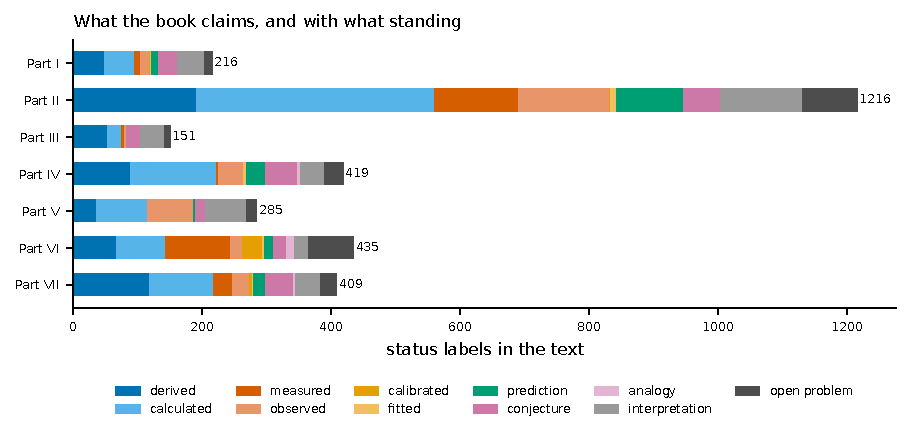
\includegraphics[width=\textwidth]{figures/part5/fig_status_summary.pdf}
\captionof{figure}{Status labels in the text of each Part, counted from the chapter sources: derived, calculated, measured, observed, calibrated, fitted, prediction, conjecture, analogy, interpretation and open problem. Recomputed from the sources by the figure script. \calc}\label{fig:status_summary}
\end{minipage}\end{center}

The order in the title is the half of the accounting that is easiest to see and hardest to measure: every system that persists spends energy
to hold what it has written against the thermal noise of its own surface. A cell that stops holding its pattern stops being that cell. \interp{}
If that holds, the same physics that reads the sky can read the health of a cell long before a disease shows itself, and can tell an engineer
where a qubit or a chip is losing what it writes. The book is offered to everyone who wants to take that further.
